%%%%%%%%%%%%%%%%%%%%%%%%%%%%%%%%%%%%%%%%%%%%%%%%%%%%%%%%%%
\section{Representation}
\label{sec:representation}
%%%%%%%%%%%%%%%%%%%%%%%%%%%%%%%%%%%%%%%%%%%%%%%%%%%%%%%%%%

\begin{figure}[t!]
   \center
   {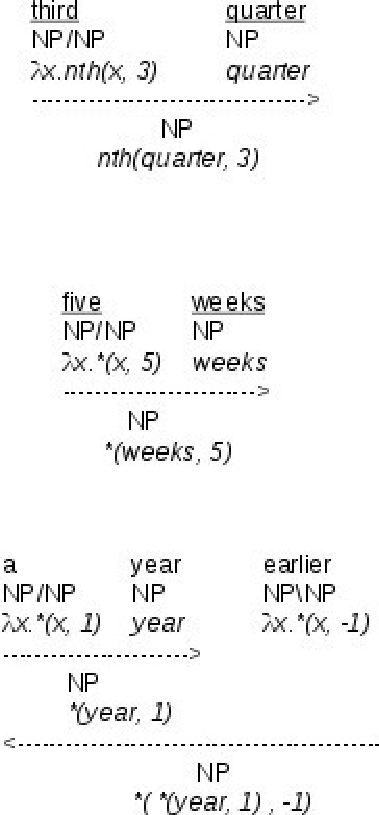
\includegraphics[width=0.5\columnwidth]{fig/lexiconExample3.pdf}}
   \caption{Above we can see three example parses. Each of these parses represents a base parse for the given temporal phrase. We can see how the base parse is built from the individual categories drawn from the lexicon. In the first example, we are parsing the phrase \emph{third quarter}. The entries in the lexicon that are being used in this parse are $\lambda x.nth(x,3)$ and $quarter$, which correspond to \emph{third} and \emph{quarter}, respectively. These combine to create the base parse for the first phrase, $nth(quarter,3)$. 
The second example is very similar to the frist. However, the third example first does forward composition (combining $\lambda x*(x,1)$ with $year$) then does backward composition (combining $\lambda x.*(x,-1)$ with $*(year,1)$). 
The first context-independent parse, $nth(quarter,3)$ represents the sequence of all third quarters, which needs additional logic to be correctly ground to a single third quarter. The second parse, $*(weeks, 5)$, can be fully ground to a duration of five weeks without needing an additional context step. The third parse, $*(*(year,1),-1)$, can't actually be ground to a date at all without additional contextual information. 
   } 
   \label{fig:lexiconExample}
\end{figure}


%This section: CCG representation, including types, the grammar.
In this section, we first define our type system, then discuss our lexicon, then describe how we parse. Our system takes a three-step parsing approach. First, we use a CCG parser to build a set base parses for each temporal phrase in isolation (where each base parse is referred to a a context-independent parse). Then, for each context-independent parse, we deterministically build five context-dependent parses. Once we select a single parse from the set of candidate context-depndent parses (a process which we discuss in section~\ref{Learning}), we execute the parse to ground to a final representation.

%%%%%%%%%%%%%%%%%%%%%%%%%%%%%%%%%%%%%%%%%%%%%%%%%%%%%%%%%%
\subsection{Types within CCG}
\label{sec:CCGtypes}
%%%%%%%%%%%%%%%%%%%%%%%%%%%%%%%%%%%%%%%%%%%%%%%%%%%%%%%%%%
We define five types in our representation below.

\begin{definition}[Range]
A range is a period between two times. For example, \emph{June 13th, 2013}, \emph{today}, and \emph{1987} all ground to ranges. Ranges also include general past and future references, such as the resolution of the phrase \emph{in the future} or \emph{previously}.
\end{definition}

\begin{definition}[Sequence] 
A sequence represents an infinite sequence of ranges. For example, \emph{each Thursday} grounds to a range. The duration between each range in a sequence is the same. In the example \emph{each Thursday}, there is a week between each range. Sequences are represented as under-specified ranges. If we were interested in grounding the phrase \emph{June 13th, 2013}, we first ground \emph{June 13th} to the sequence of all June 13ths, which we could represent as XXXX-6-13, i.e. June 13th of an unspecified year, then intersect that sequence with the range 2013.
\end{definition}

\begin{table*}[tp]
\begin{tabular}{|l|l|l|}
  \hline
  \textbf{Function} & \textbf{Description} & \textbf{Type} \\
  \hline \hline
  intersect & Finds the intersection of two sequences & $f:s* -> s$ \\
  \hline
  * & Multiplies a duration by a number & $f:d,n -> d$ \\
  \hline
  nth x of y & Finds the \emph{nth} sequence within y (quarter of year, etc)& $f:d,n -> s$ \\
  \hline
  next & Returns the range immediately following the document time & $f:s,r -> s$; $f:d,r -> s$ \\
  \hline
  this & Returns the range within which the document time falls & $f:s,r -> s$; $f:d,r -> s$ \\
  \hline
  previous & Returns the range immediately before the document time & $f:s,r -> s$; $f:d,r -> s$ \\
  \hline
  temproalReference & Grounds duration/sequence based on previous temporal phrase & $f:s -> s$; $f:d -> s$ \\
  \hline
\end{tabular}
  \caption{A list of all of the predicates in our logic of airity greater than zero.}
  \label{table:functions}
\end{table*}

\begin{definition}[Duration]
A duration is a period of time with no specified start or end dates. For example, \emph{two months}, \emph{three years}, and \emph{one day} all ground to durations of time. 
\end{definition}

\begin{definition}[Number]
Numbers only appear in logical forms, never in fully executed output. Numbers are necessary when grounding durations, such as \emph{4 years}, \emph{1 hour}, or \emph{3 weeks}. 
\end{definition}

\begin{definition}[Functional Types]
There are a number of functional types, all of arity less than or equal to two. The complete set is listed in~\ref{table:functions}.
\end{definition}



\begin{table}
 \begin{tabular}{|l|l|}
  \hline
  \textbf{Type} & \textbf{Examples} \\
  \hline \hline
  Range & 1987, 2013-06-15, Past, 1990-Q2, etc. \\
  Sequence & Friday, third quarter, each week, etc. \\
  Duration & Hour, Day, Week, Month, etc. \\
  \hline
 \end{tabular}
 \caption{A list of some examples for each of the three primary zero-arity predicates.}
\end{table}

%%%%%%%%%%%%%%%%%%%%%%%%%%%%%%%%%%%%%%%%%%%%%%%%%%%%%%%%%%
\subsection{Lexicon}
%%%%%%%%%%%%%%%%%%%%%%%%%%%%%%%%%%%%%%%%%%%%%%%%%%%%%%%%%%

A CCG is defined by a lexicon and set of combinators. In this work, we use standard forward and backward application with a hand-built lexicon to build our base parses. See ~\ref{fig:lexiconExample} for an example.




%%%%%%%%%%%%%%%%%%%%%%%%%%%%%%%%%%%%%%%%%%%%%%%%%%%%%%%%%%
\subsection{Pasing Using CCG}
%%%%%%%%%%%%%%%%%%%%%%%%%%%%%%%%%%%%%%%%%%%%%%%%%%%%%%%%%%
First, for each temporal phrase in our dataset, we use a CKY parser to get a set of CCG logical forms. These are built only from the phrase itself, and don't take any additional information into account. Some ranges can be fully ground without looking at the context in which they appear, such as \emph{June 6th, 2013}. Similarly, durations such as \emph{five weeks} or \emph{a year} don't need to look at surrounding context to be executed to a final form. However, the majority of phrases do require some context to ground fully. Phrases such as \emph{Friday} are parsed to logic that represent a sequences, in this case the sequence of all Fridays. To ground phrases such as those to a single range, we need to look at context.
%%%%%%%%%%%%%%%%%%%%%%%%%%%%%%%%%%%%%%%%%%%%%%%%%%%%%%%%%%
\subsection{Building Context-Dependent Parse}
%%%%%%%%%%%%%%%%%%%%%%%%%%%%%%%%%%%%%%%%%%%%%%%%%%%%%%%%%%


From each context-independent logical form we get from the base CCG parser, we use a deterministic process to build a set of five context-dependent logical forms. These represent the five possible groundings of each of our base parses. 

For fully-sepcified ranges and for durations, we don't actually need to change the logical form, so the frist of the the context-dependent logical forms is an unchanged version of the context-independent logical form. 

Sequences often represent an infinite number of ranges, such as $nth(quarter,3)$. We can ground these sequences to one of three ranges: The range before the document was published, the range after the document was published, or the range during which the document was published. These three groundings are represented by the next three logical forms, which are constructed by applying the three predicates $\lambda x.last(x, publicationTime)$, $\lambda x.this(x, publicationTime)$, and $\lambda x.next(x, publicationTime)$ to the base parse. We make the assumption that if someone were referring to a range other than the one before, during, or after the document was published that they would refer to it using a fully-specified range, instead of requiring resolution through context. This assumption allows us to only need these three additional context-dependent logical forms to ground any sequence, and matches our intuitions about how language is used. 

Finally, for a class of temporal phrases that refer to a previously uttered temporal phrase, such as \emph{a year earlier}, we build a logical form that grounds the current phrase based on the previous one by applying the predicate $\lambda x.temporalReference(x)$ to the base parse. An example of this process is shown in~\ref{fig:contextIndependentLogicalForms}.
\begin{figure*}[b]
   \center
   {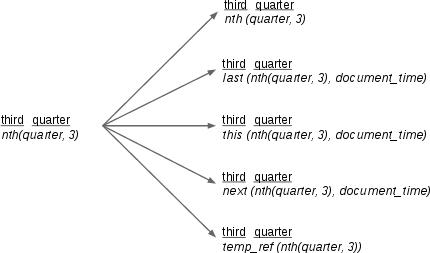
\includegraphics[width=1.2\columnwidth]{fig/context-independentLogicalForms.jpg}}
   \caption{The creation of the five context-dependent logical forms from one context-independent logical form. This determinisitic process always generates five logical forms by applying five predicates to the base parse. First, a predicate $\lambda x.x$, which always returns its argument. Next, three predicates to ground a single range out of a sequence, $\lambda x.last(x, documentTime)$, $\lambda x.this(x, documentTime)$, and $\lambda x.next(x, documentTime)$. Finally, a predicate $\lambda x.temporalReference(x)$ that resolves $x$ based on the previously uttered temproal phrase.
   } 
   \label{fig:contextIndependentLogicalForms}
\end{figure*}

\begin{figure}[t!]
   \center
   {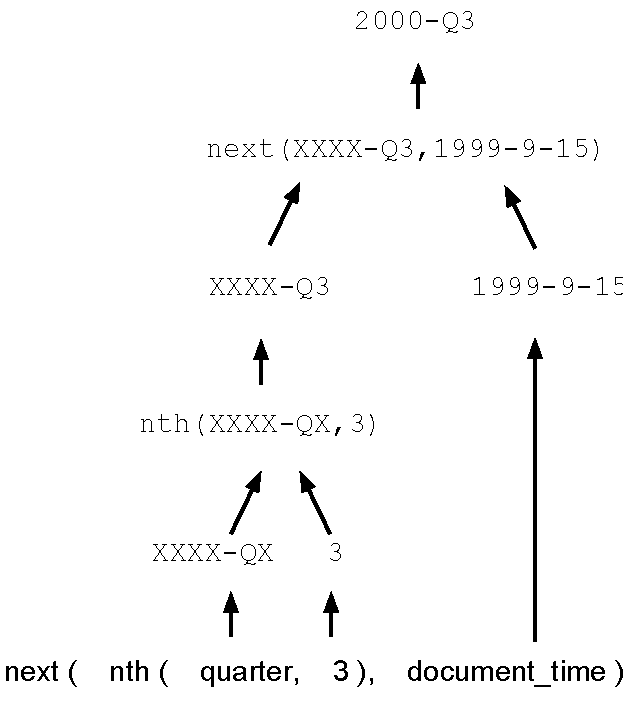
\includegraphics[width=.85\columnwidth]{fig/executionExample.pdf}}
   \caption{An example execution from a context-dependent logical form to a fully ground date, built from the phrase \emph{third quarter}. Assumes the document the phrase appeared in was published September 15th, 1999. We recursively execute the logic \texttt{next(nth(quarter,3),documentTime)} to the final \emph{value} \texttt{2000-Q3}. To do this, first we ground the zero-arity predicates, \texttt{quarter}, \texttt{3}, and \texttt{documentTime}. Then, we use those to ground the predicates with airity greater than zero, \texttt{nth} and \texttt{next}.
   } 
   \label{fig:executionExample}
\end{figure}

%%%%%%%%%%%%%%%%%%%%%%%%%%%%%%%%%%%%%%%%%%%%%%%%%%%%%%%%%%
\subsection{Execution}
%%%%%%%%%%%%%%%%%%%%%%%%%%%%%%%%%%%%%%%%%%%%%%%%%%%%%%%%%%
Once we have built a set of candidate context-dependent logical forms, we then execute them to fully ground the temporal phrases. Our execution is a deterministic process, done by walking the logic recursively. Within our logical forms, the no-argument predicates ground to a date or duration directly, while the predicates that take arguments act as functions over those ground dates or durations. Evaluating the logic recursively, we start with the outermost predicate and work our way in. 

















